% ICLR full-width motivation figure; generated by scripts/plot_student_t_tails.py.
\begin{figure*}[t]
  \centering
  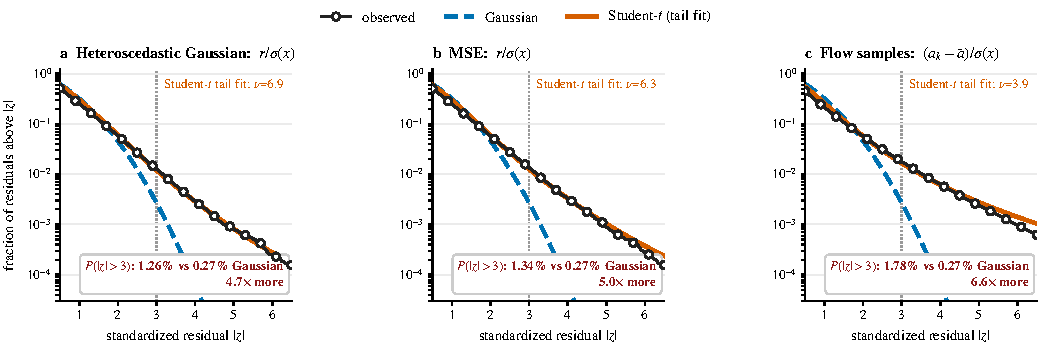
\includegraphics[width=\textwidth]{analysis/paper/student_t_tails/fig_student_t_tails.pdf}
  \caption{\textbf{Residuals stay heavy-tailed after input-dependent scaling.} Fraction of coordinates with standardized residual magnitude above $|z|$ on the same
  1{,}728 WidowX demonstration states (six continuous action channels, eight-step
  chunks), against the standard normal and a Student-$t$ fitted to the tail beyond one standard deviation. Every quantity is divided by a learned
  state-local scale $\sigma(x)$, the per-state scale of a heteroscedastic Gaussian head, then by each coordinate's RMS,
  and rescaled to unit RMS. \textbf{(a)} The heteroscedastic Gaussian head's own residual. \textbf{(b)} The residual of an
  MSE head. \textbf{(c)} The deviation of each of 16 Flow samples from their per-state mean. Annotations give the share
  of events beyond $3\sigma$ relative to the Gaussian 0.27\%. Removing the state-dependent scale leaves a tail that is
  4.7 to 6.6 times heavier than Gaussian; this remaining tail is what the Student-$t$ likelihood models.}
  \label{fig:student-t-tails}
\end{figure*}
